%
% File: chap01.tex
% Author: Victor F. Brena-Medina
% Description: Introduction chapter where the biology goes.
%
\let\textcircled=\pgftextcircled
\chapter{Result Analysis and Discussion}
\label{chap:implementation}
In this chapter, the result analysis and discussion have been clarified. For discussion convenience, there are a total of 4 sub-chapters under chapter 4, which we introduced. In section 4.1, we discussed experimental tools; in section 4.2, we discussed result; in section 4.3, we discussed the discussion part.

\vspace{150mm}
%\vspace{2mm}

%=======
\section{Experimental Elements}
\label{sec:sec4_1}
There are different types of implementation tools for deep learning. Most of the tools can be used for thesis paper code. When we want to get our thesis outcome, it must need for any researchers. Most of the time, \textbf{Jupyter Notebook, Google Colab, and Kaggle Notebook} are used for the implementation of any thesis paper code. With this tool, we can easily run our code without any problems.\\

We have used \textbf{Jupyter Notebook} in our experiment. It is an open-source, web-based interactive computing platform widely used for data analysis, machine learning, and scientific research. Jupyter Notebook allows us to create and share documents containing live code, equations, visualizations, and narrative text. It supports a variety of programming languages, with Python being the most popular. For implementation, no internet connection is required when running it locally, but it can also be hosted on cloud platforms. Jupyter Notebook offers seamless integration with many computational libraries, making it a versatile tool for executing and documenting experiments. The flexibility to visualize data, run code interactively, and document results in a single environment makes Jupyter Notebook a preferred choice for researchers and developers.

\section{Result}
\label{sec:sec4_2}
This study applied a two-stage methodology for BdSL classification, utilizing ResNet-50 for feature extraction and evaluating two classifiers SVM (Support Vector Machine) and CNN (Convolutional Neural Network) for the final classification job. After extract feature using ResNet-50 SVM train must faster. And dense layer also works well.

\begin{figure}[H]
\centering
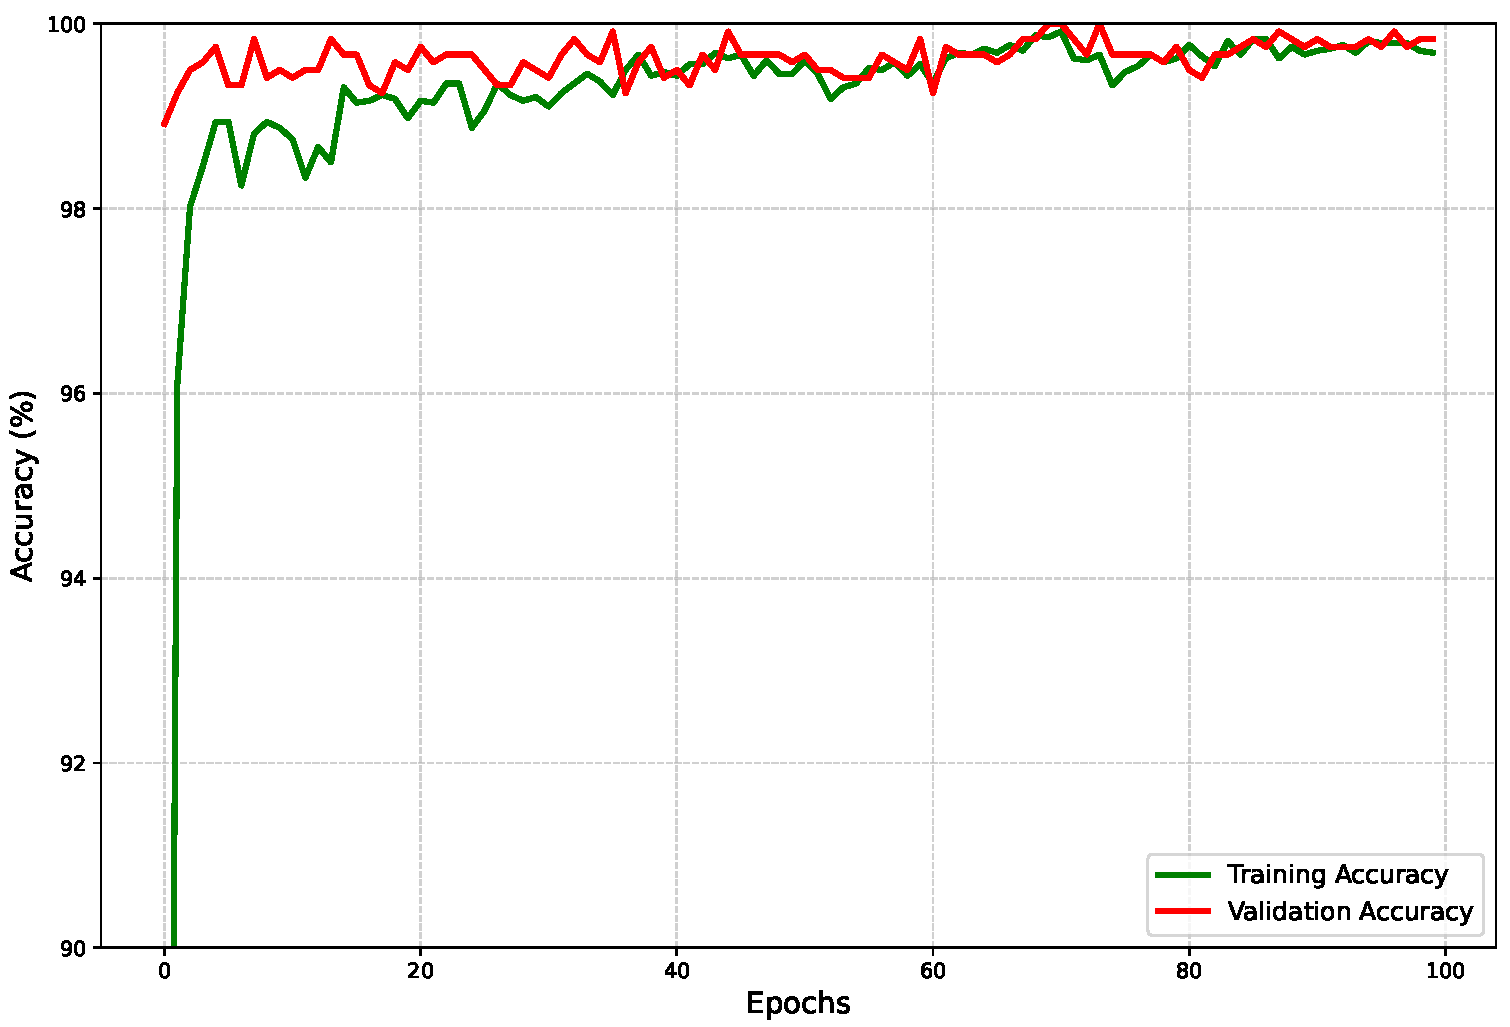
\includegraphics[height=8cm]{./fig/accuracy_curve.pdf} 
\centering
\caption{Accuracy Curve (ResNet-50 + Dense Layer)}
\label{Accuracy_Curve}
\end{figure}

\begin{figure}[H]
\centering
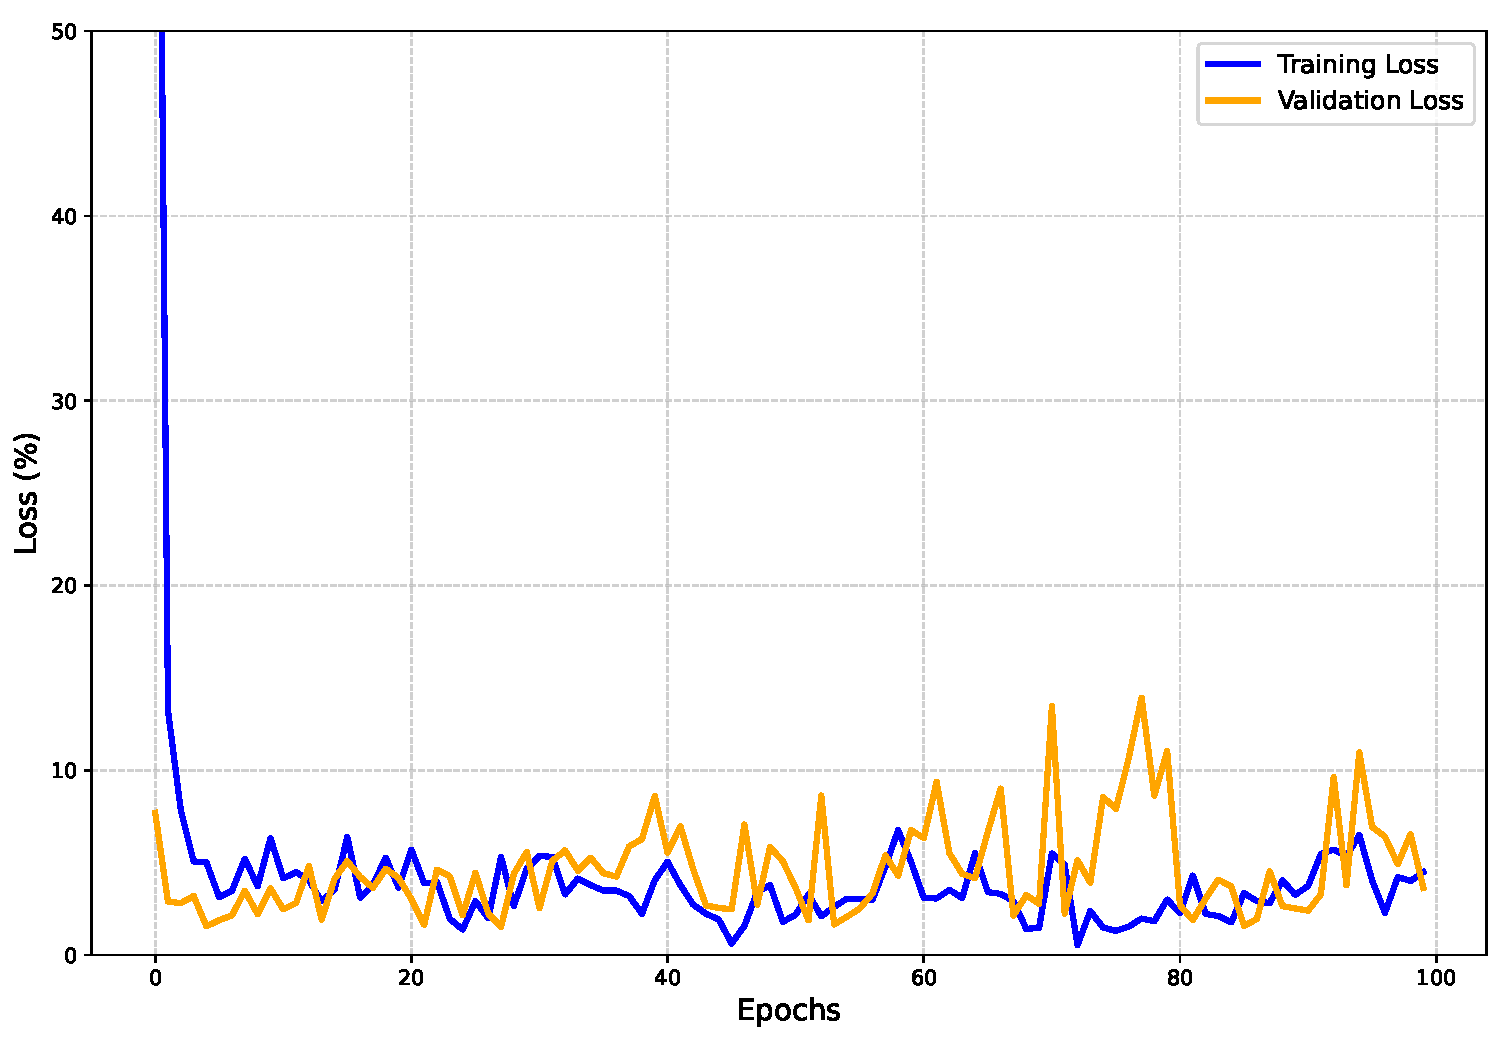
\includegraphics[height=8cm]{./fig/loss_curve.pdf} 
\centering
\caption{Loss Curve (ResNet-50 + Dense Layer)}
\label{Loss_Curve}
\end{figure}

\subsection{Classification Report}
\label{sec:sec4_3_2}
In analyzing the performance of a classification model, a classification report is very useful. The purpose of this report is to indicate the important metrics of model performance including precision, recall and F1 score for analysis.\\

We define precision as the fraction of these instances with positive predicted labels. It is an indicator of the model's accuracy in identifying true positives and is calculated as follows:\\

TP = True Positives; FN = False Negatives; TN = True Negatives; FP = False Positives.

\begin{center}
$\text{Precision} = \frac{TP}{TP + FP}$
\end{center}

However, recall is how many actual positive instances the model identified as positive instances. It's the fraction of all positive cases that the model can identify as positive. Recall is calculated as: 

\begin{center}
    $\text{Recall} = \frac{TP}{TP + FN}$
\end{center}

The F1 score evaluates precision and recall simultaneously and returns an indicator of the balance of these two quantities. It is the mean harmonic calculus between precision and recall, implementation with both metrics in a single score. The F1-score is calculated as:

\begin{center}
    $\text{F1 Score} = \frac{2 \times Precision \times Recall}{Precision + Recall}$
\end{center}

Precision and recall are two essential metrics in BdSL classification. High precision means we have few false positives by reducing some predicted positive cases. The importance of the recall lies in the fact that a high recall will result in the model finding the most optimistic cases, hence the most important to avoid miss classification. In BdSL classification, the F1 Score is also very important. This parameter matters at a time when a very high number of positive detections indicates a very low false positive level because it ensures that the performance of the model is valid. The following show the classification report of the respective methods:

\vspace{8mm}
\begin{table}[h]
\centering
\begin{tabular}{|c|c|c|c|c|}
\hline
\textbf{Methodology} & \textbf{Accuracy} & \textbf{Precision} & \textbf{Recall} & \textbf{F1-Score} \\
\hline
\textbf{ResNet-50 + SVM} & \textbf{99.7\%} & \textbf{1.00} & \textbf{1.00} & \textbf{1.00} \\
\hline
ResNet-50 + Dense Layer & 99.5\% & 1.00 & 1.00 & 1.00 \\
\hline
\end{tabular}
\caption{Classification Report.}
\label{tab:classification_report}
\end{table}

\newpage
\subsection{Per Class Performance}
\label{sec:sec4_3_3}

\begin{figure}[H]
\centering
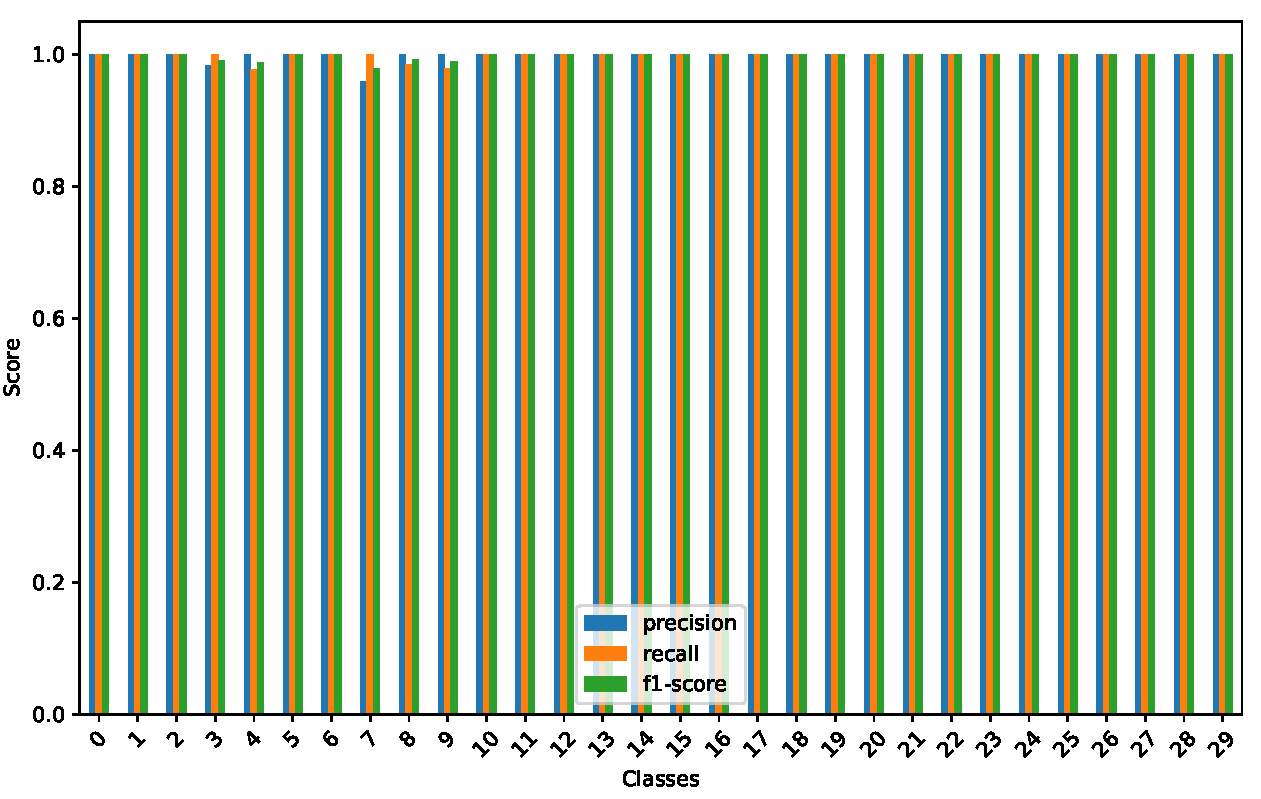
\includegraphics[height=8cm]{./fig/per_class.pdf} 
\centering
\caption{Per-Class Performance Metrics (ResNet-50 + SVM)}
\label{per_class_svm}
\end{figure}

\begin{figure}[H]
\centering
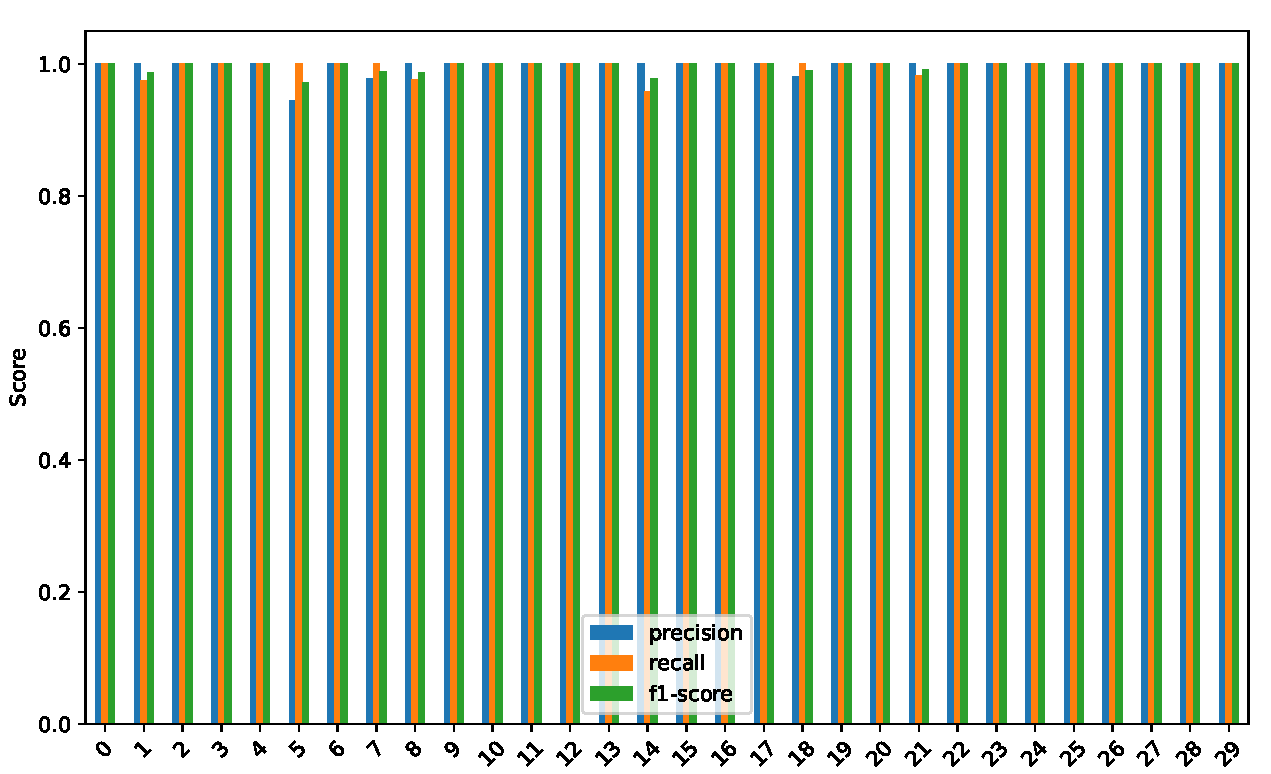
\includegraphics[height=8cm]{./fig/per_class2.pdf} 
\centering
\caption{Per-Class Performance Metrics (ResNet-50 + Dense Layer)}
\label{per_class_dense}
\end{figure}

\newpage
\subsection{Confusion Matrix}
\label{sec:sec4_3_4}
The confusion matrix is a very useful way of evaluating a classification model’s performance. It also presents a table between the predicted class and actual class of each test instance. The matrix is divided into four components: true positives, false positives, and true negatives, and false negatives.The following show the two confusion matrices of our methods:

\begin{figure}[H]
\centering
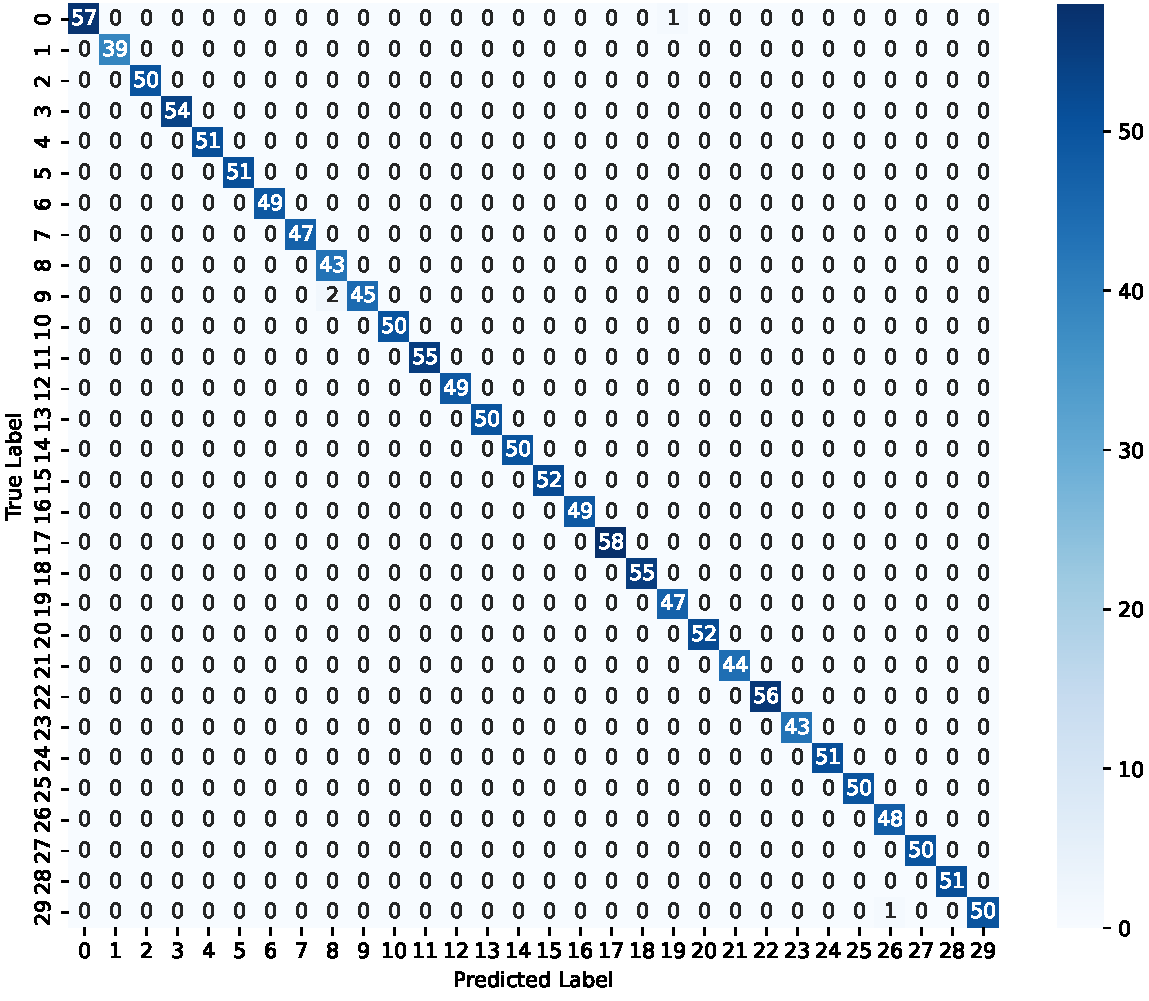
\includegraphics[height=8cm]{./fig/confusion_matrix.pdf} 
\centering
\caption{Confusion Matrix (ResNet-50 + SVM)}
\label{Confusion_matrix_svm}
\end{figure}

\begin{figure}[H]
\centering
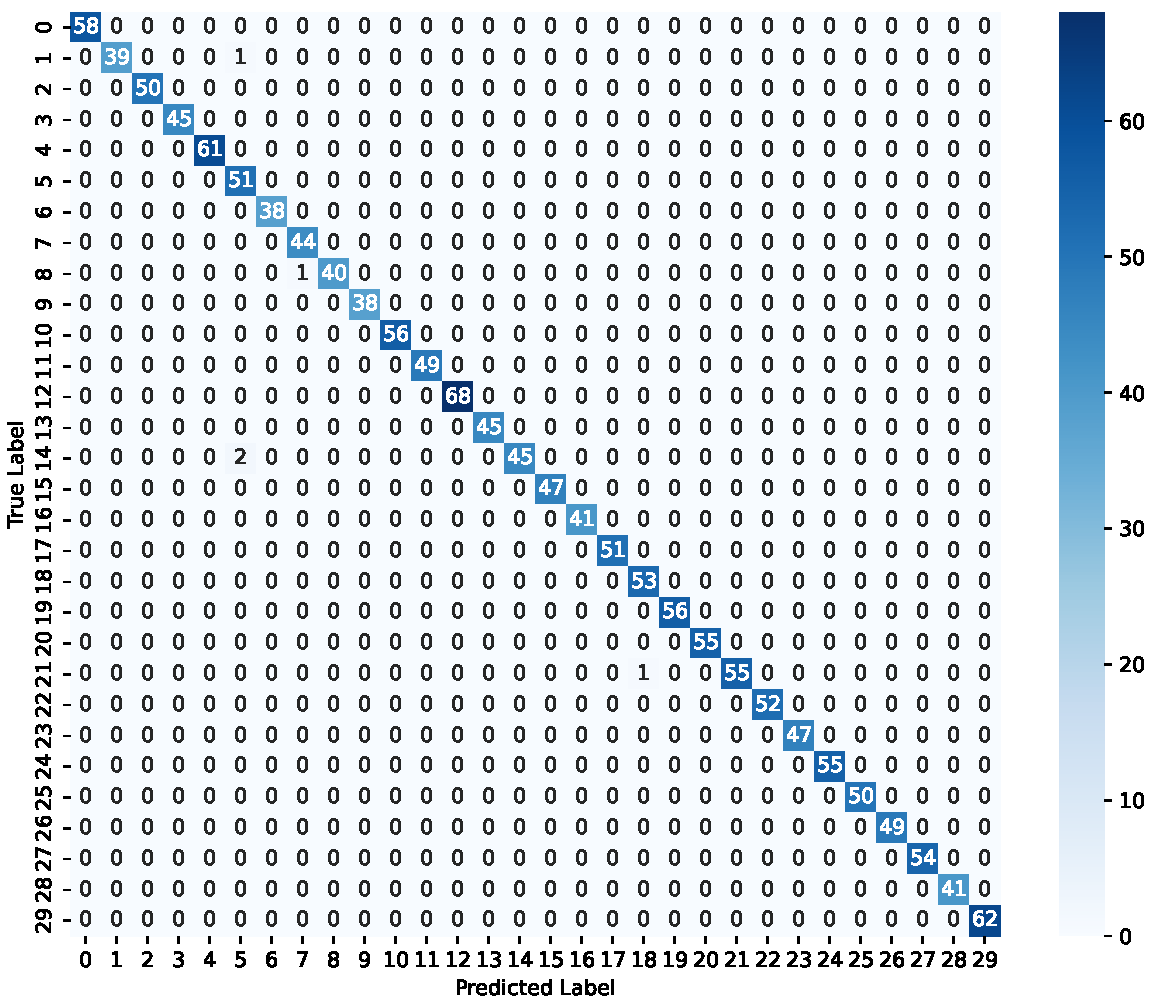
\includegraphics[height=8cm]{./fig/confusion_matrix_2.pdf} 
\centering
\caption{Confusion Matrix (ResNet-50 + Dense Layer)}
\label{Confusion_matrix_dense}
\end{figure}

\newpage
\section{Discussion}
\label{sec:sec4_4_5}